\documentclass[../main.tex]{subfiles}

\begin{document}

\chapter{UML Diagrams}\label{appendix-uml_diagrams}
Sequence and class diagrams of the software module.

\vspace{2em}

\begin{figure}[h]
    \centering
    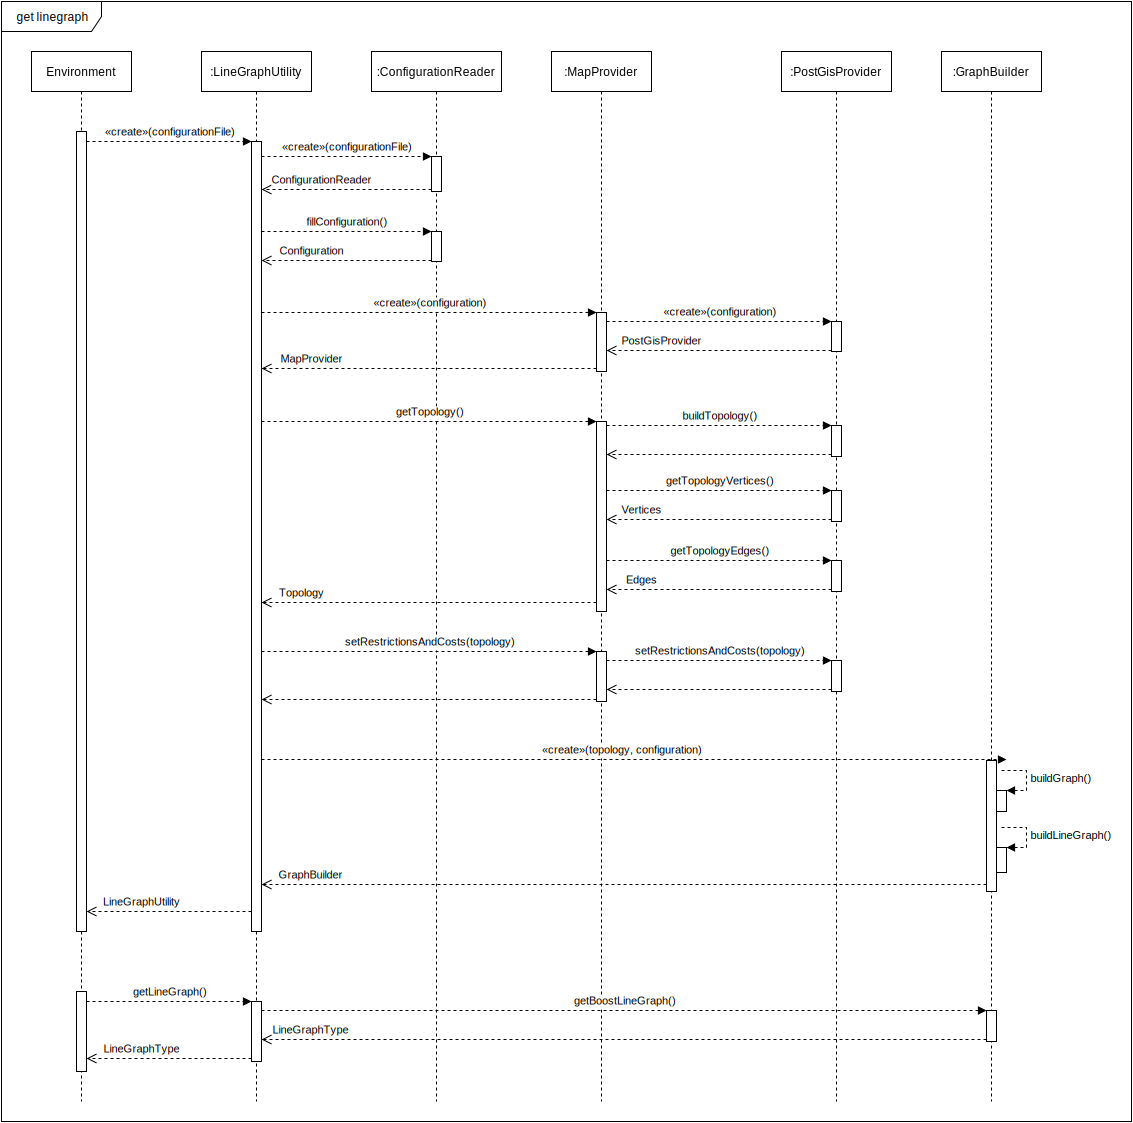
\includegraphics[width=1.1\linewidth]{uml_seq_get_linegraph}
    \caption{Sequence diagram of main use case to get a line graph.}
    \label{fig:appendix_uml_seq_get_linegraph}
\end{figure}

\clearpage
\begin{figure}[H]
    \centering
    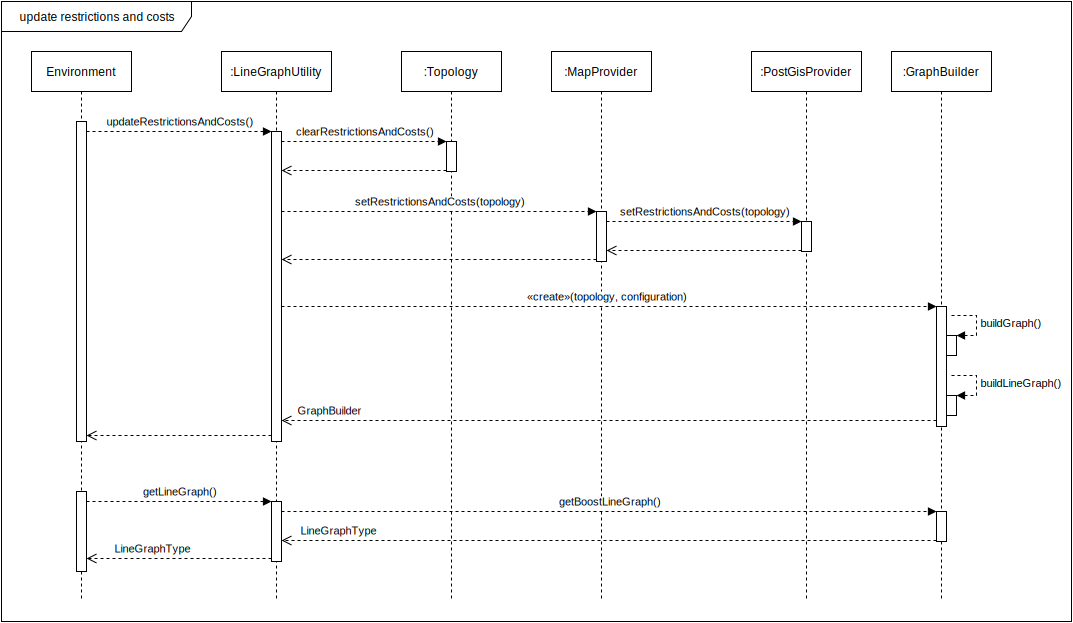
\includegraphics[width=1.1\linewidth]{uml_seq_update_costs}
    \caption{Sequence diagram of updating costs and restrictions on a topology.}
    \label{fig:appendix_uml_seq_update_costs}
\end{figure}

\clearpage
\begin{figure}[H]
    \centering
    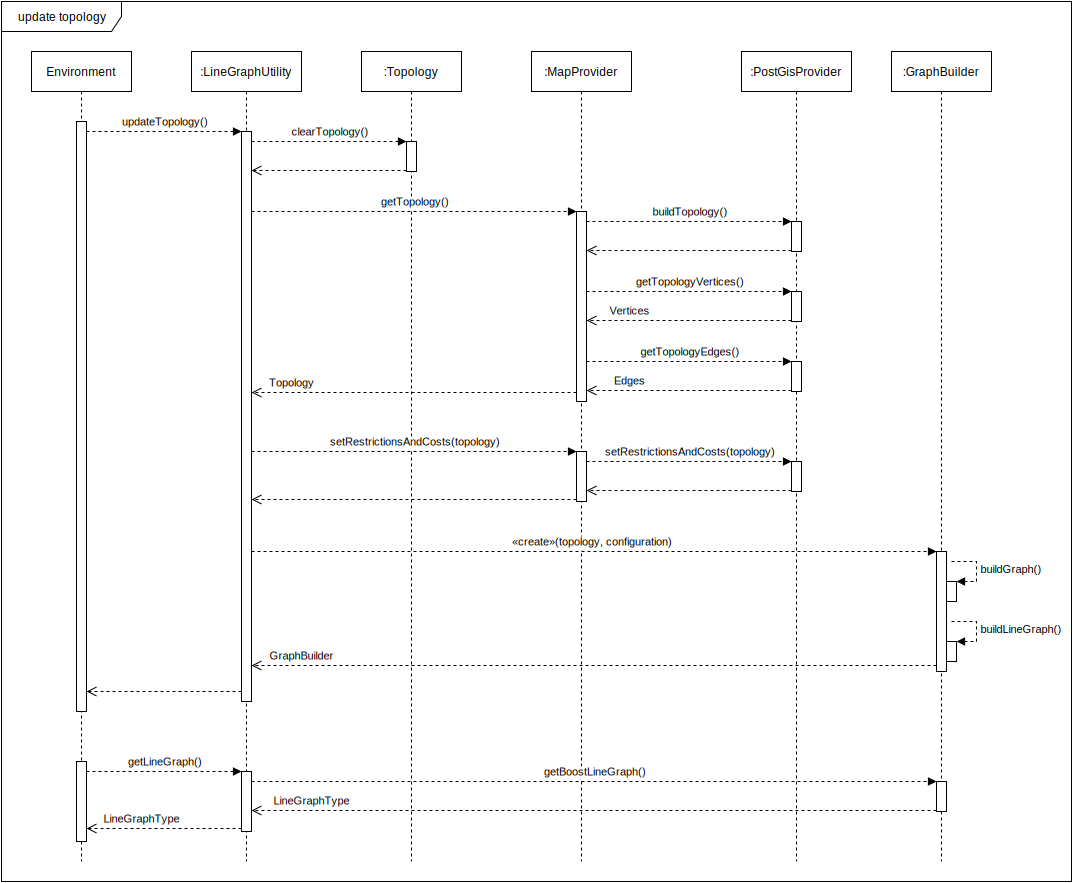
\includegraphics[width=1.1\linewidth]{uml_seq_update_topology}
    \caption{Sequence diagram of updating the topology.}
    \label{fig:appendix_uml_seq_update_topology}
\end{figure}

\clearpage
\begin{sidewaysfigure}[h!]
    \centering
    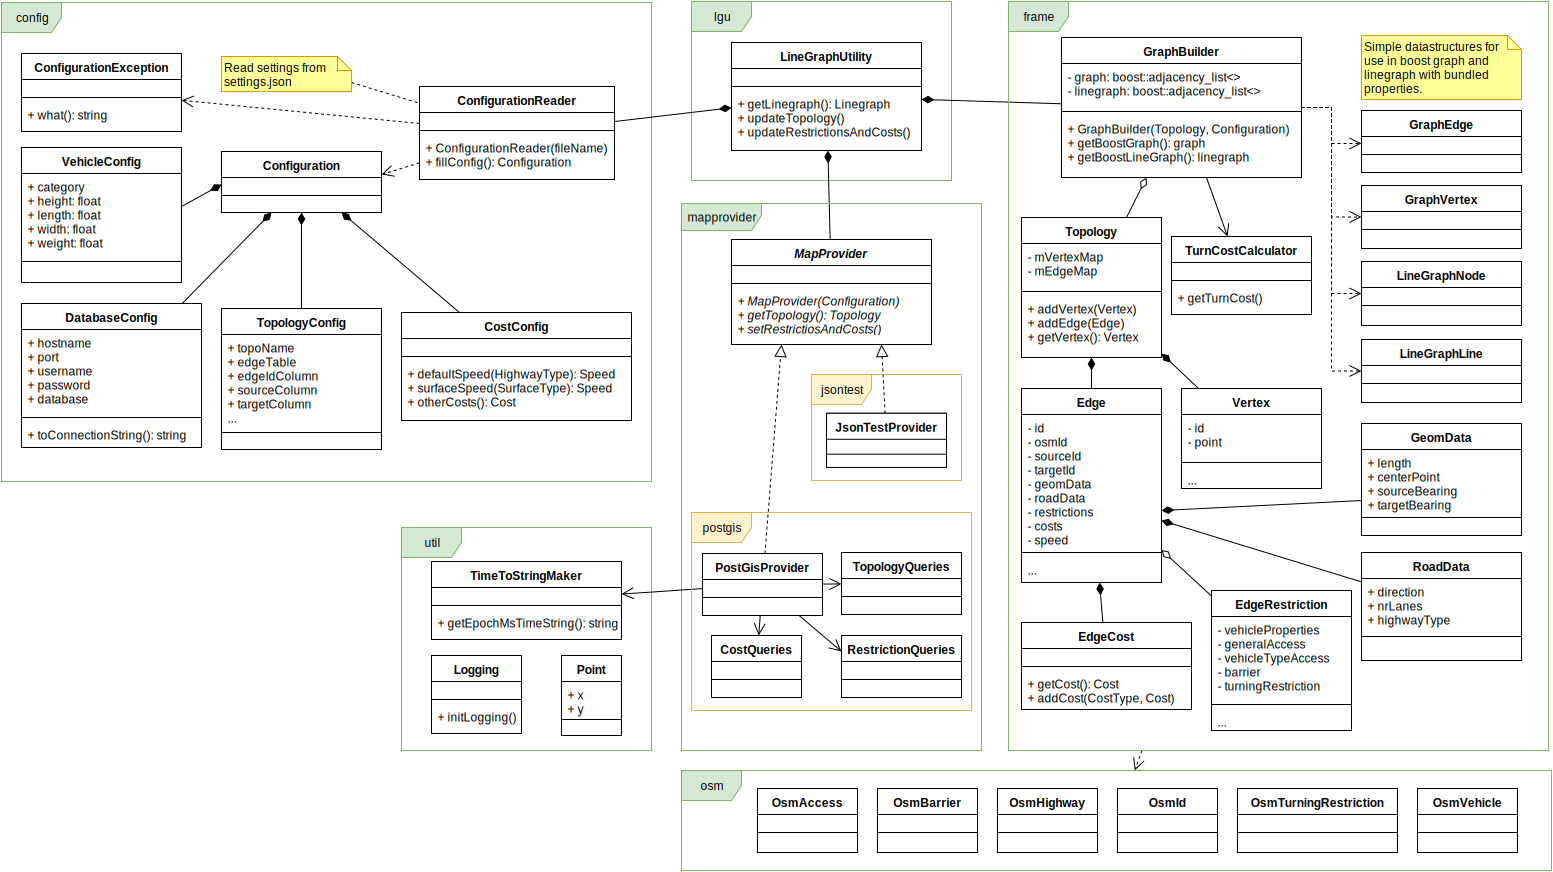
\includegraphics[width=\linewidth]{uml_class_lgu}
    \caption{Class diagram of the \textit{line graph utility}.}
    \label{fig:appendix_uml_class_lgu}
\end{sidewaysfigure}

\end{document}
